\documentclass{article}
\usepackage{fancyhdr}
\usepackage{amsthm}
\usepackage{etoolbox}
\usepackage{verbatim}
\usepackage{enumerate}
\usepackage{amsmath}
\usepackage{algorithmicx}
\usepackage{algorithm}
\usepackage{algpseudocode}
\usepackage{fancybox}
\usepackage{tikz}


	
\pagestyle{fancy}
\title{Chapter 6}
\author{Michelle Bodnar, Andrew Lohr}

\newcounter{curnum}
\setcounter{curnum}{0}

\newtheorem{th1}{Exercise} 
\newcommand{\calH}{\mathcal{H}}
\newcommand{\calX}{\mathcal{X}}
\newcommand{\calA}{\mathcal{A}}
\newcommand{\calY}{\mathcal{Y}}

\begin{document}
\maketitle

\noindent\textbf{Exercise 6.1-1}\\

At least $2^h$ and at most $2^{h+1}-1$. Can be seen because a complete binary tree of depth $h-1$ has $\Sigma_{i=0}^{h-1} 2^i = 2^h-1$ elements, and the number of elements in a heap of depth $h$ is between the number for a complete binary tree of depth $h-1$ exclusive and the number in a complete binary tree of depth $h$ inclusive.\\

\noindent\textbf{Exercise 6.1-2}\\

Write $n = 2^m-1 + k$ where $m$ is as large as possible.  Then the heap consists of a complete binary tree of height $m-1$, along with $k$ additional leaves along the bottom. The height of the root is the length of the longest simple path to one of these $k$ leaves, which must have length $m$.  It is clear from the way we defined $m$ that $m = \lfloor \lg n \rfloor$. \\

\noindent\textbf{Exercise 6.1-3}\\

If there largest element in the subtee were somewhere other than the root, it has a parent that is in the subtree. So, it is larger than it's parent, so, the heap property is violated at the parent of the maximum element in the subtree\\

\noindent\textbf{Exercise 6.1-4}\\

The smallest element must be a a leaf node.  Suppose that node $x$ contains the smallest element and $x$ is not a leaf.  Let $y$ denote a child node of $x$.  By the max-heap property, the value of $x$ is greater than or equal to the value of $y$.  Since the elements of the heap are distinct, the inequality is strict.  This contradicts the assumption that $x$ contains the smallest element in the heap. \\


\noindent\textbf{Exercise 6.1-5}\\

Yes, it is. The index of a child is always greater than the index of the parent, so the heap property is satisfied at each vertex.\\

\noindent\textbf{Exercise 6.1-6}\\

No, the array is not a max-heap.  7 is contained in position 9 of the array, so its parent must be in position 4, which contains 6.  This violates the max-heap property. \\

\noindent\textbf{Exercise 6.1-7}\\

It suffices to show that the elements with no children are exactly indexed by $\{\lfloor n/2\rfloor+1, \ldots, n\}$. Suppose that we had an $i$ in this range. It's childeren would be located at $2i$ and $2i+1$ but both of these are $\ge 2 \lfloor n/2\rfloor +2 > n$ and so are not in the array. Now, suppose we had an element with no kids, this means that $2i$ and $2i+1$ are both $>n$, however, this means that $i > n/2$. This means that $i\in \{\lfloor n/2\rfloor+1, \ldots, n\}$.\\

\noindent\textbf{Exercise 6.2-1}\\

$
\begin{array}{|c|c|c|c|c|c|c|c|c|c|c|c|c|c|}
\hline
27&17&3&16&13&10&1&5&7&12&4&8&9&0\\
\hline
27&17&10&16&13&3&1&5&7&12&4&8&9&0\\
\hline
27&17&10&16&13&8&1&5&7&12&4&3&9&0\\
\hline
\end{array}
$\\

\noindent\textbf{Exercise 6.2-2}\\

\begin{algorithm}
\caption{MIN-HEAPIFY(A,i)}
\begin{algorithmic}[1]
\State $l=LEFT(i)$ 
\State $r=RIGHT(i)$
\If{$l \leq A.heap-size$ and $A[l] < A[i]$}
	\State $smallest = l$
\Else{ $smallest = i$}
\EndIf
\If{$r \leq A.heap-size$ and $A[r] < A[smallest]$}
	\State $smallest = r$
\EndIf
\If{$smallest \neq i$}
	\State exchange $A[i]$ with $A[smallest]$
	\State MAX-HEAPIFY($A, smallest$)
\EndIf
\end{algorithmic}
\end{algorithm}

The running time of MIN-HEAPIFY is the same as that of MAX-HEAPIFY. \\


\noindent\textbf{Exercise 6.2-3}\\

The array remains unchanged since the if statement on line line 8 will be false.\\

\noindent\textbf{Exercise 6.2-5}\\
Iterative Max Heapify$(A,i)$
\begin{algorithm}
\begin{algorithmic}
\While{$i<A$.heap-size}
\State $l =$LEFT$(i)$
\State $r =$LEFT$(i)$
\State $largest = i$
\If{$l\le A$.heap-size and $A[l]>A[i]$}
\State $largest =l$
\EndIf
\If{$l\le A$.heap-size and $A[r]>A[i]$}
\State $largest =r$
\EndIf
\If{$largest \neq i$}
\State exchange $A[i]$ and $A[largest]$
\Else \Return A
\EndIf
\EndWhile
\State \Return A
\end{algorithmic}
\end{algorithm}\\

\noindent\textbf{Exercise 6.2-4}\\

If $i > A.heap-size/2$ then $l$ and $r$ will both exceed $A.heap-size$ so the if statement conditions on lines 3 and 6 of the algorithm will never be satisfied.  Therefore $largest = i$ so the recursive call will never be made and nothing will happen. This makes sense because $i$ necessarily corresponds to a leaf node, so MAX--HEAPIFY shouldn't alter the heap. \\

\noindent\textbf{Exercise 6.3-1}\\

$
\begin{array}{|c|c|c|c|c|c|c|c|c|}
\hline
5&3&17&10&84&19&6&22&9\\
\hline
5&3&17&22&84&19&6&10&9\\
\hline
5&3&19&22&84&17&6&10&9\\
\hline
5&84&19&22&3&17&6&10&9\\
\hline
84&5&19&22&3&17&6&10&9\\
\hline
84&22&19&5&3&17&6&10&9\\
\hline
84&22&19&10&3&17&6&5&9\\
\hline
\end{array}
$\\

\noindent\textbf{Exercise 6.3-2}\\

If we had started at 1, we wouldn't be able to guarantee that the max-heap property is maintained.  For example, if the array $A$ is given by [2,1,1,3] then MAX-HEAPIFY won't exchange 2 with either of it's children, both 1's.  However, when MAX-HEAPIFY is called on the left child, 1, it will swap 1 with 3.  This violates the max-heap property because now 2 is the parent of 3. \\

\noindent\textbf{Exercise 6.3-3}\\

All the nodes of height $h$ partition the set of leaves into sets of size between $2^{h-1}+1$ and $2^h$, where all but one is size $2^h$. Just by putting all the children of each in their own part of trhe partition. Recall from 6.1-2 that the heap has height $\lfloor \lg(n)\rfloor$, so, by looking at the one element of this height (the root), we get that there are at most $ 2^{\lfloor \lg(n)\rfloor}$ leaves. Since each of the vertices of height $h$ partitions this into parts of size at least $2^{h-1}+1$, and all but one corresponds to a part of size $2^h$, we can let $k$ denote the quantity we wish to bound, so,
\[
(k-1)2^h + k(2^{h-1}+1) \le 2^{\lfloor \lg(n) \rfloor} \le n/2
\]
so
\[
k \le  \frac{n+2^h}{2^{h+1} + 2^{h}+1 }\le \frac{n}{2^{h+1}} \le \left\lceil \frac{n}{2^{h+1}}\right\rceil
\]\\
%We know from 6.1-2 that a n-element heap must have height $\lfloor \lg(n) \rfloor$. We also know that at distance $d$ from the root, there are at most $2^d$ nodes. Since the 

\noindent\textbf{Exercise 6.4-1}\\

$
\begin{array}{|c|c|c|c|c|c|c|c|c|}
\hline
5&13&2&25&7&17&20&8&4\\
\hline
5&13&20&25&7&17&2&8&4\\
\hline
5&25&20&13&7&17&2&8&4\\
\hline
25&5&20&13&7&17&2&8&4\\
\hline
25&13&20&5&7&17&2&8&4\\
\hline
25&13&20&8&7&17&2&5&4\\
\hline
4&13&20&8&7&17&2&5&25\\
\hline
20&13&4&8&7&17&2&5&25\\
\hline
20&13&17&8&7&4&2&5&25\\
\hline
5&13&17&8&7&4&2&20&25\\
\hline
17&13&5&8&7&4&2&20&25\\
\hline
2&13&5&8&7&4&17&20&25\\
\hline
13&2&5&8&7&4&17&20&25\\
\hline
13&8&5&2&7&4&17&20&25\\
\hline
4&8&5&2&7&13&17&20&25\\
\hline
8&4&5&2&7&13&17&20&25\\
\hline
8&7&5&2&4&13&17&20&25\\
\hline
4&7&5&2&8&13&17&20&25\\
\hline
7&4&5&2&8&13&17&20&25\\
\hline
2&4&5&7&8&13&17&20&25\\
\hline
5&4&2&7&8&13&17&20&25\\
\hline
2&4&5&7&8&13&17&20&25\\
\hline
4&2&5&7&8&13&17&20&25\\
\hline
2&4&5&7&8&13&17&20&25\\
\hline
\end{array}
$\\

\noindent\textbf{Exercise 6.4-2}\\

We'll prove the loop invariant of HEAPSORT by induction:

Base case: At the start of the first iteration of the for loop of lines 2-5 we have $i=A.length$. The subarray $A[1..n]$ is a max-heap since BUILD-MAX-HEAP(A) was just called.  It contains the $n$ smallest elements, and the empty subarray $A[n+1..n]$ trivially contains the 0 largest elements of $A$ in sorted order.\\

Suppose that at the start of the $i^{th}$ iteration of of the for loop of lines 2-5, the subarray $A[1..i]$ is a max-heap containing the $i$ smallest elements of $A[1..n]$ and the subarray $A[i+1..n]$ contains the $n-i$ largest elements of $A[1..n]$ in sorted order. Since $A[1..i]$ is a max-heap, $A[1]$ is the largest element in $A[1..i]$. Thus it is the $(n-(i-1))^{th}$ largest element from the original array since the $n-i$ largest elements are assumed to be at the end of the array.  Line 3 swaps $A[1]$ with $A[i]$, so $A[i..n]$ contain the $n-i+1$ largest elements of the array, and $A[1..i-i]$ contains the $i-1$ smallest elements.  Finally, MAX-HEAPIFY is called on $A,1$.  Since $A[1..i]$ was a max-heap prior to the iteration and only the elments in positions 1 and $i$ were swapped, the left and right subtrees of node 1, up to node $i-1$, will be max-heaps.  The call to MAX-HEAPIFY will place the element now located at node 1 into the correct position and restore the max-heap property so that $A[1..i-1]$ is a max-heap.  This concludes the next iteration, and we have verified each part of the loop invariant.  By induction, the loop invariant holds for all iterations.\\

After the final iteration, the loop invariant says that the subarray $A[2..n]$ contains the $n-1$ largest elements of $A[1..n]$, sorted.  Since $A[1]$ must be the $n^{th}$ largest element, the whole array must be sorted as desired. \\

\noindent\textbf{Exercise 6.4-3}\\

If it's already sorted in increasing order, doing the build max heap-max-heap call on line 1 will take $\Theta(n\lg(n))$ time. There will be $n$ iterations of the for loop, each taking $\Theta(\lg(n))$ time because the element that was at position $i$ was the smallest and so will have $\lfloor \lg(n)\rfloor$ steps when doing max-heapify on line 5. So, it will be $\Theta(n\lg(n))$ time.

If it's already sorted in decreasing order, then the call on line one will only take $\Theta(n)$ time, since it was already a heap to begin with, but it will still take $n\lg(n)$ peel off the elements from the heap and re-heapify. \\

\noindent\textbf{Exercise 6.4-4}\\

Consider calling HEAPSORT on an array which is sorted in decreasing order.  Every time $A[1]$ is swapped with $A[i]$, MAX-HEAPIFY will be recursively called a number of times equal to the height $h$ of the max-heap containing the elements of positions 1 through $i-1$, and has runtime $O(h)$.  Since there are $2^k$ nodes at height $k$, the runtime is bounded below by
\[ \sum_{i=1}^{\lfloor\lg n\rfloor} 2^i \log(2^i) =  \sum_{i=1}^{\lfloor\lg n\rfloor} i2^i = 2 + (\lfloor\lg n\rfloor - 1)2^{\lfloor\lg n\rfloor} = \Omega(n\lg n).\]



\noindent\textbf{Exercise 6.4-5}\\

Since the call on line one could possibly take only linear time (if the input was already a max-heap for example), we will focus on showing that the for loop takes n log n time. To do this, we will show that the re-heapifying takes at least $\lg(n)$ steps on average. In particular, since what was in the $i$'th position before the swap was less than all it's parents, each time an element is put on the top and re-heapafied, when it takes $i$  steps, it will guarentee that all the children of the depth $i$ subheap rooted at it will take one additional step. This gets us the desired bound.\\
%needs more work

\noindent\textbf{Exercise 6.5-1}\\

$
\begin{array}{|c|c|c|c|c|c|c|c|c|c|c|c|}
\hline
15&13&9&5&12&8&7&4&0&6&2&1\\
\hline
1&13&9&5&12&8&7&4&0&6&2&\\
\hline
13&1&9&5&12&8&7&4&0&6&2&\\
\hline
13&12&9&5&1&8&7&4&0&6&2&\\
\hline
13&12&9&5&6&8&7&4&0&1&2&\\
\hline
\end{array}
$\\

\noindent\textbf{Exercise 6.5-2}\\

The following sequence of pictures shows how 10 is inserted into the heap, then swapped with parent nodes until the max-heap property is restored.  The node containing the new key is heavily shaded.

\begin{enumerate}
\item  Original heap:

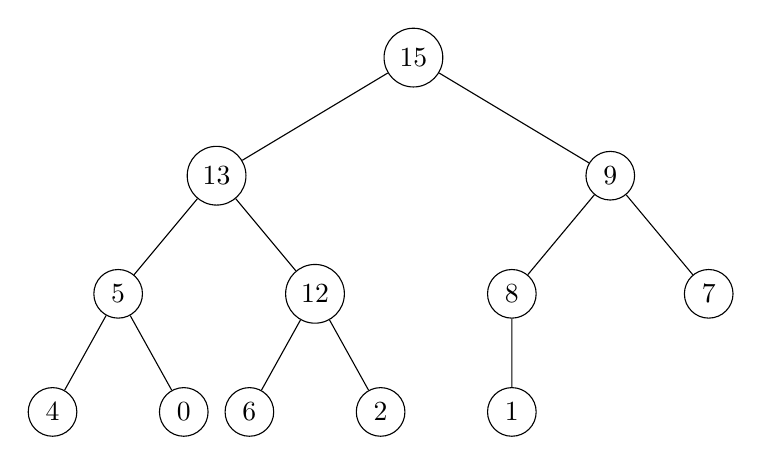
\begin{tikzpicture}[level/.style={sibling distance=50mm/#1}]
\node [circle,draw] (z){15}
  child {node [circle,draw] (a) {13}
    child {node [circle,draw] (b) {5}
      child {node [circle,draw] (c) {4}
	}
      child {node [circle,draw] (d) {0}
	}
    }
    child {node [circle,draw] (g) {12}
	child {node [circle,draw] (c) {6}}
      child {node [circle,draw] (d) {2}}
  }}
  child {node [circle,draw] (a) {9}
    child {node [circle,draw] (b) {8}
      child {node [circle,draw] (c) {1}
	}
    }
    child {node [circle,draw] (g) {7}
  }};
\end{tikzpicture}
\item MAX-HEAP-INSERT(A,10) is called, so we first append a node assigned value $-\infty$:

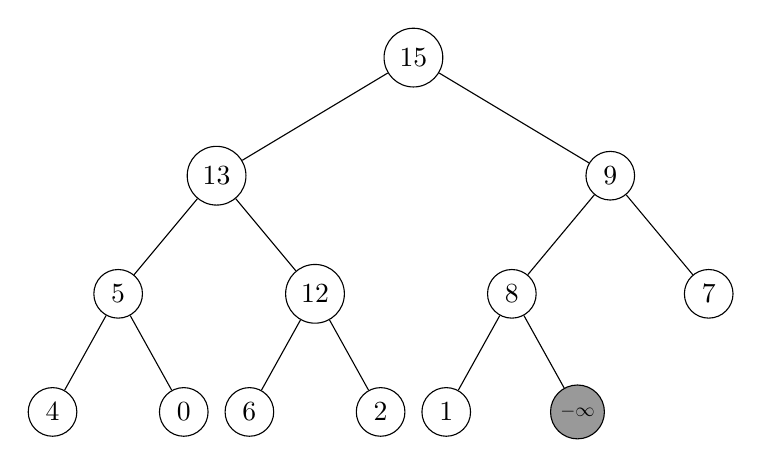
\begin{tikzpicture}[level/.style={sibling distance=50mm/#1}]
\node [circle,draw] (z){15}
  child {node [circle,draw] (a) {13}
    child {node [circle,draw] (b) {5}
      child {node [circle,draw] (c) {4}
	}
      child {node [circle,draw] (d) {0}
	}
    }
    child {node [circle,draw] (g) {12}
	child {node [circle,draw] (c) {6}}
      child {node [circle,draw] (d) {2}}
  }}
  child {node [circle,draw] (a) {9}
    child {node [circle,draw] (b) {8}
      child {node [circle,draw] (c) {1}
	}
	child{node [circle,draw,scale=.7, fill=black!40] (c) {$-\infty$}}
    }
    child {node [circle,draw] (g) {7}
  }};
\end{tikzpicture}
\item The key value of the new node is updated:

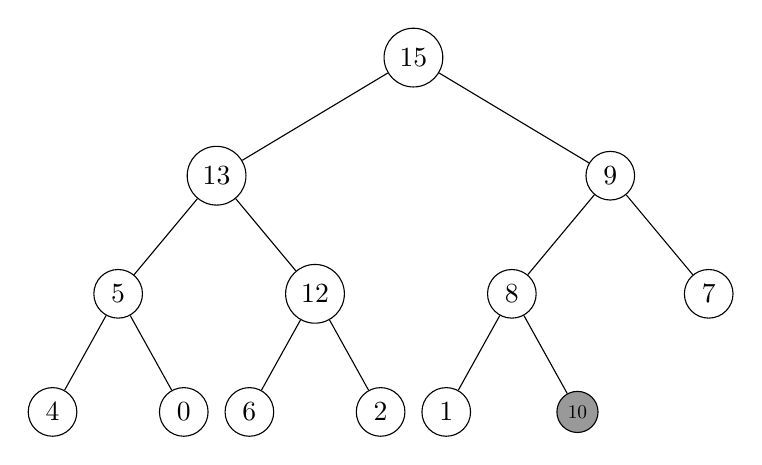
\begin{tikzpicture}[level/.style={sibling distance=50mm/#1}]
\node [circle,draw] (z){15}
  child {node [circle,draw] (a) {13}
    child {node [circle,draw] (b) {5}
      child {node [circle,draw] (c) {4}
	}
      child {node [circle,draw] (d) {0}
	}
    }
    child {node [circle,draw] (g) {12}
	child {node [circle,draw] (c) {6}}
      child {node [circle,draw] (d) {2}}
  }}
  child {node [circle,draw] (a) {9}
    child {node [circle,draw] (b) {8}
      child {node [circle,draw] (c) {1}
	}
	child{node [circle,draw,scale=.7, fill=black!40] (c) {10}}
    }
    child {node [circle,draw] (g) {7}
  }};
\end{tikzpicture}
\item Since the parent key is smaller than 10, the nodes are swapped:

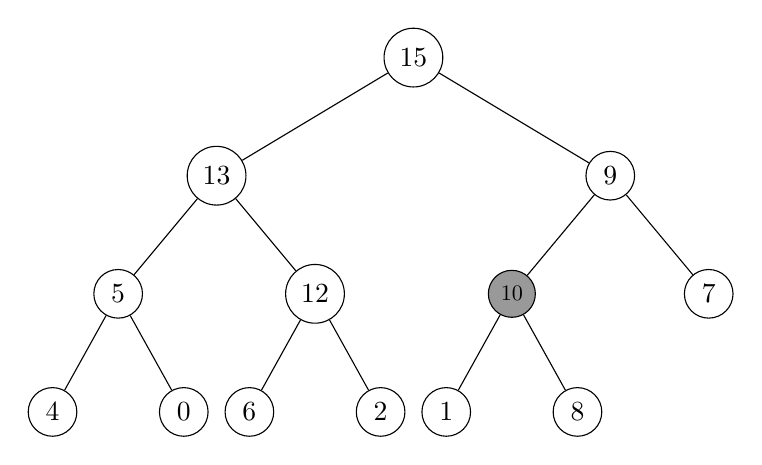
\begin{tikzpicture}[level/.style={sibling distance=50mm/#1}]
\node [circle,draw] (z){15}
  child {node [circle,draw] (a) {13}
    child {node [circle,draw] (b) {5}
      child {node [circle,draw] (c) {4}
	}
      child {node [circle,draw] (d) {0}
	}
    }
    child {node [circle,draw] (g) {12}
	child {node [circle,draw] (c) {6}}
      child {node [circle,draw] (d) {2}}
  }}
  child {node [circle,draw] (a) {9}
    child {node [circle,draw ,scale=.8, fill=black!40] (b) {10}
      child {node [circle,draw] (c) {1}
	}
	child{node [circle,draw] (c) {8}}
    }
    child {node [circle,draw] (g) {7}
  }};
\end{tikzpicture}
\item Since the parent node is smaller than 10, the nodes are swapped:

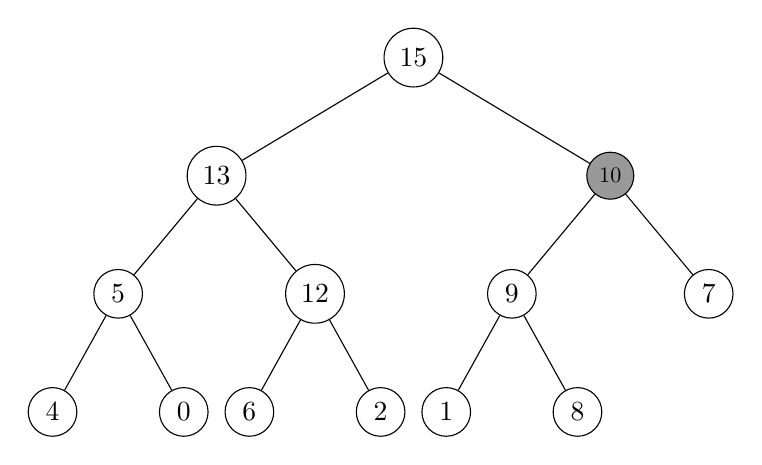
\begin{tikzpicture}[level/.style={sibling distance=50mm/#1}]
\node [circle,draw] (z){15}
  child {node [circle,draw] (a) {13}
    child {node [circle,draw] (b) {5}
      child {node [circle,draw] (c) {4}
	}
      child {node [circle,draw] (d) {0}
	}
    }
    child {node [circle,draw] (g) {12}
	child {node [circle,draw] (c) {6}}
      child {node [circle,draw] (d) {2}}
  }}
  child {node [circle,draw ,scale=.8, fill=black!40] (a) {10}
    child {node [circle,draw] (b) {9}
      child {node [circle,draw] (c) {1}
	}
	child{node [circle,draw] (c) {8}}
    }
    child {node [circle,draw] (g) {7}
  }};
\end{tikzpicture}
\end{enumerate}

\noindent\textbf{Exercise 6.5-3}\\

Heap-Minimum(A)
\begin{algorithm}
\begin{algorithmic}[1]
\State \Return A[1]
\end{algorithmic}
\end{algorithm}

Heap-Extract-Min(A)
\begin{algorithm}
\begin{algorithmic}[1]
\If{A.heap-size $<1$}
\State Error ``heap underflow''
\EndIf
\State $min = A[1]$
\State $A[1] = A[A.heap-size]$
\State $A.heap-size --$
\State Min-heapify(A,1)
\State \Return min 
\end{algorithmic}
\end{algorithm}

Heap-decrease-key(A,i,key)
\begin{algorithm}
\begin{algorithmic}[1]
\If{key > A[i]}
\State Error ``new key larger than old key''
\EndIf
\State $A[i] =key$
\While{$i>1$ and $A[Parent(i)] < A[i]$}
\State exchange $A[i]$ with $A[Parent(i)]$
\State $i = Parent(i)$
\EndWhile
\end{algorithmic}
\end{algorithm}

Min-Heap-Insert(A,key)
\begin{algorithm}
\begin{algorithmic}[1]
\State $A.heap-size ++$
\State $A[A.heap-size] = \infty$
\State Heap-Decrease-Key(A,A.heap-size,key)
\end{algorithmic}
\end{algorithm}\\



\noindent\textbf{Exercise 6.5-5}\\

Initially, we hve a heap and then only change the value at $i$ to make it larger. This can't invalidate the ordering between $i$ and it's children, the only other thing that needs to be related to $i$ is that $i$ is less than it's parent, which may be false. Thus we have the invariant is true at initalization. Then, when we swap $i$ with its parent if it is larger, since it is larger than it's parent, it must also be larger than it's sibling, also, since it's parent was initally above its kids in the heap, we know that it's parent is larger than it's kids. The only relation in question is then the new $i$ and it's parent. At termination, $i$ is the root, so it has no parent, so the heap property must be satisfied everywhere.\\


\noindent\textbf{Exercise 6.5-7}\\

Have a field in the structure that is just a count of the total number of elements ever added. When adding an element, use the current value of that counter as the key.\\



\noindent\textbf{Exercise 6.5-9}\\

Construct a min heap from the heads of each of the $k$ lists. Then, to find the next element in the sorted array, extract the minimum element (in $O\lg(k)$ time). Then, add to the heap the next element from the shorter list from which the extracted element originally came (also $O(\lg(k))$ time). Since finding the next element in the sorted list takes only at most $O(\lg(k))$ time, to find the whole list, you need $O(n\lg(k))$ total steps. \\



\noindent\textbf{Problem 6-1}\\

\begin{enumerate}[a.]
\item
They do not. Consider the array $A =\langle 3,2,1,4,5\rangle$. If we run Build-Max-Heap, we get $\langle 5,4,1,3,2\rangle$. However, if we run Build-Max-Heap', we will get $\langle 5,4,1,2,3\rangle$ instead.
\item
Each insert step takes at most $O(\lg(n))$, since we are doing it $n$ times, we get a bound on the runtime of $O(n\lg(n))$.
\end{enumerate}
\noindent\textbf{Problem 6-3}\\
\begin{enumerate}[a.]
\item
$
\begin{array}{|c|c|c|c|}
\hline
2&3&4&5\\
\hline
8&9&12&14\\
\hline
16&\infty&\infty&\infty\\
\hline
\infty&\infty&\infty&\infty\\
\hline
\end{array}
$

\item
For every $i,j$, $Y[1,1] \le Y[i,1] \le Y[i,j]$. So, if $Y[1,1] = \infty$, we know that $Y[i,j]=\infty$ for every $i,j$. This means that no elements exist. If $Y$ is full, it has no elements labeled $\infty$, in particular, the element $Y[m,n]$ is not labeled $\infty$.
\item
Extract-Min(Y,i,j), extracts the minimum value from the young tableau $Y'$ obtained by $Y'[i',j'] = Y[i'+i-1,j'+j-1]$. Note that in running this algorithm, several accesses may be made out of bounds for $Y$, define these to return $\infty$. No store operations will be made on out of bounds locations.
\begin{algorithm}
\begin{algorithmic}[1]
\State $min = Y[i,j]$
\If{ $Y[i,j+1] = Y[i+1,j]= \infty$}
\State $Y[i,j] = \infty$
\State \Return min
\EndIf
\If{$Y[i,j+1] < Y[i+1,j]$ }
\State $Y[i,j] = Y[i,j+1]$
\State $Y[i,j+1] = min$
\State \Return Extract-min(y,i,j+1)
\Else
\State $Y[i,j] = Y[i+1,j]$
\State $Y[i+1,j] = min$
\State \Return Extract-min(y,i+1,j)
\EndIf
\end{algorithmic}
\end{algorithm}
Since the largest value of $i+j$ that this can be called with is $n+m$, and this quantity must increase by one for each call, we have that the runtime is bounded by $n+m$.

\item
Insert(Y,key)
\begin{algorithm}
\begin{algorithmic}[1]
\State$i=m$, $j=n$
\State $Y[i,j] = key$
\While{$Y[i-1,j] > Y[i,j]$ or $Y[i,j-1] >Y[i,j]$}
\If{$Y[i-1,j] < Y[i,j-1]$}
\State Swap $Y[i,j]$ and $Y[i,j-1]$
\State $j--$
\Else
\State Swap $Y[i,j]$ and $Y[i-1,j]$
\State $i--$
\EndIf
\EndWhile
\end{algorithmic}
\end{algorithm}
Since $i+j$ is decreasing at each step, starts as $n+m$ and is bounded by $2$ below, we know that this program has runtime $O(n+m)$.
\item
Place the $n^2$ elements into a Young Tableau by calling the algorithm from part d on each. Then, call the algorithm from part c $n^2$ to obtain the numbers in increasing order. Both of these operations take time at most $2n\in O(n)$, and are done $n^2$ times, so, the total runtime is $O(n^3)$
\item
Find(Y,key). Let Check(y,key,i,j) mean to return true if $Y[i,j]=key$, otherwise do nothing
\begin{algorithm}
\begin{algorithmic}
\State$ i =j= 1$
\While{$Y[i,j] <key$ and $i<m$}
\State Check(Y,key,i,j)
\State i++
\EndWhile
\While{$i>1$ and $j<n$}
\State Check(i,j)
\If{$Y[i,j]<key$}
\State j++
\Else
\State i--
\EndIf
\EndWhile
\State \Return false
\end{algorithmic}
\end{algorithm}
\end{enumerate}


\end{document}